\chapter{Einleitung}\label{kap:Einleitung}
Im Verbundprojekt Autonome Systeme soll ein Fertigungsprozess mit autonom agierenden Robotern automatisiert werden. Dazu befinden sich acht Stationen mit jeweils zwei Arbeitsplätzen und einem Platz zum Lesen oder Schreiben von RFID-Tags im Versuchsaufbau. Station 1 repräsentiert dabei das Rohteillager und Station 8 das Fertigteillager. Die Arbeitsschritte werden durch Aufenthalt der Werkstücke für eine bestimmte Zeit an den Arbeitsplätzen simuliert. Je nach Produkt, das hergestellt werden soll, variiert die Anzahl, Reihenfolge, und Bearbeitungszeit der Stationen. Zum Transport der Werkstücke zwischen den Stationen werden autonom agierende Roboter mit einer Greifzange eingesetzt. Die Navigation der Roboter wird mit Hilfe von ermittelten Positionsdaten realisiert, die mit Kameras ermittelt werden. Als Software wird, für die Programmierung der Roboter, Matlab/Simulink eingesetzt. Für die Auftragsplanung wird Qt verwendet. Das Speichern der Produktionsdaten erfolgt über eine MySQL-Datenbank und die RFID-Technologie wird mit CODESYS angesteuert.

\section{Aufgaben Gewerk 1}

Das Gewerk 1 ist zuständig für:

\begin{itemize}
    \item die Fertigungsplanung,
    \item die Visualisierung des Fertigungsprozesses,
    \item das Beschreiben und Auslesen der RFID-Tags auf den Werkstücken und
    \item das Ablegen aller produktionsrelevanten Daten in der MySQL-Datenbank.
\end{itemize}

Die Fertigungsplanung soll die über das visuelle HMI eingegebenen Aufträge verwalten und den Robotern ihre Aufträge zuweisen. Die Visualisierung soll die Roboter und ihre Position so wie die Arbeitsstationen darstellen. Über die Visualisierung soll ebenfalls die Auftragseingabe stattfinden und der aktuelle Fortschritt eines Auftrags abgebildet werden. Ebenso ist die vom Fertigungsrechner mit Hilfe der RFID-Technologie durchgeführte Verfolgung der Werkstücke darzustellen.

Der Fertigungsrechner soll die RFID-Tags der Werkstücke mit Hilfe der RFID-Schreib-Lese-Köpfe beschreiben, beziehungsweise auslesen, um so eine Verfolgung der Werkstücke durch den Produktionsprozess zu ermöglichen. Auf dem Fertigungsrechner befindet sich auch der Server für die MySQL-Datenbank, die alle produktionsrelevanten Daten speichert und sowohl vom Programm für die RFID-Technologie, als auch von der Fertigungsplanung lesend und schreibend angesprochen wird.

\section{Gesamtkonzept Gewerk 1}

Das Gesamtkonzept von Gewerk 1 ist in Abbildung \ref{fig:Gesamtkonzept} dargestellt.

\begin{figure}[htb]
	    \centering
	    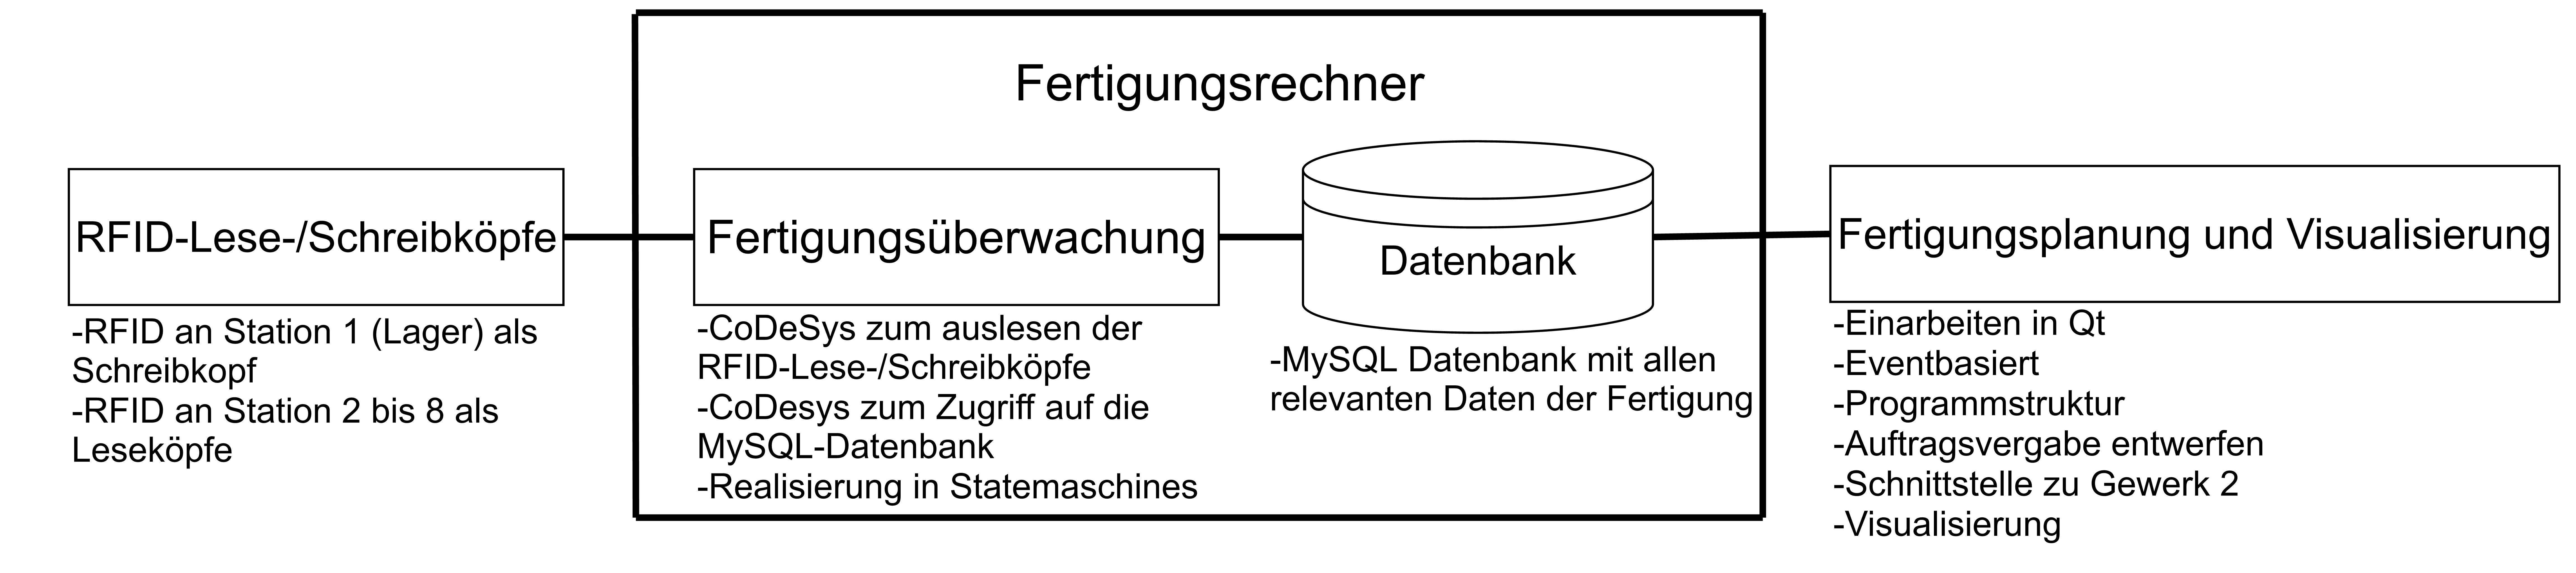
\includegraphics[width=1\linewidth]{Bilder/Konzept2.png}
        \caption{Gesamtkonzept von Gewerk 1}
        \label{fig:Gesamtkonzept}
\end{figure}

Die Fertigungsplanung und die Visualisierung werden in einem gemeinsamen Programm, dass mit Qt geschrieben wurde, realisiert. Die Fertigungsplanung empfängt für die Visualisierung über Ethernet per UDP/IP die Daten des Navigationsrechners. Die Kommunikation mit den Robotern wird ebenso von der Fertigungsplanung über WLAN per UDP/IP realisiert. Die Kommunikation zur Datenbank, die sich auf dem Fertigungsrechner befindet, findet über Ethernet statt. Die RFID-Schreib-Lese-Köpfe werden über ein Interface mittels Profibus-DP an den Fertigungsrechner angeschlossen. Das Programm zum Auslesen, beziehungsweise Beschreiben, der RFID-Tags wird mit CODESYS geschrieben und läuft auf einer Soft-SPS auf dem Fertigungsrechner. An Station 1 werden die RFID-Tags des Werkstücks beschrieben und an den Stationen 2 bis 8 ausgelesen. Über SQL4Automation kann das Programm auf die Datenbank lesend und schreibend zugreifen. In der Datenbank sind alle für den Produktionsprozess relevanten Daten abgelegt. Es handelt sich um eine relationale MySQL-Datenbank. Die Datenbank dient auch zur Kommunikation zwischen dem CODESYS-Programm auf dem Fertigungsrechner und der Fertigungsplanung. 

